\documentclass[UTF8]{ctexart}

\usepackage{subfiles}  

%下面的语句, 引入你的头部设置文件
\usepackage{C:/phpStorm_proj/02_myself_ID_EGO/+100_latex_all_math_sel/myPreamble} 
%必须是绝对路径,才能让各个tex在单独编译时使用到

\title{文件名}


%---------------------------------


\begin{document}
	\tableofcontents % 生成目录
	\date{} % 若不写这句, 则默认也会渲染出日期, 所以我们要手动赋空值
	\maketitle  %这行代码, 让你前面的 title, author, date生效
	
\section{离散型 : 泊松分布 (poisson distribution) : \\  $	P\left( \text{事}X=\text{想} \right) =\frac{\text{均}^{\text{想}}\cdot e^{-\text{均}}}{\text{想!}}	$}
	
	\textbf{``泊松分布"研究的是 : 在``单位时间(或空间)"内, ``随机事件发生任意次数"的概率.} \\
	
	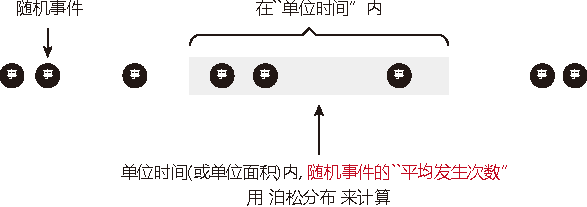
\includegraphics[width=0.7\textwidth]{/0185.pdf} \\
	
	即, ``泊松分布"是为了解决这样的问题的:单位时间内, 随机事件发生的次数, 即: 一件事发生的概率P是已知的, 但它的发生与否是随机的. 我们想要求它(即该随机事件)发生k次(或 $\geq k \text{次}, \leq k \text{次}$  等问题)的概率. \\
	
	当一个随机事件, 以固定的``平均瞬时速率$\lambda$"(或称``密度")随机且独立地出现时,那么这个事件在``单位时间(面积或体积)"内出现的次数或个数, 就近似地服从``泊松分布". \\
	\textbf{泊松分布的参数$\lambda$ : 是单位时间(或单位面积)内, 随机事件的平均发生次数.} \\
	
	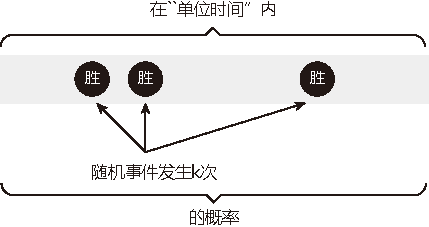
\includegraphics[width=0.55\textwidth]{/0156.pdf} \\
	
	``泊松分布" 的期望和方差, 均为$\lambda$. \\
	
	
	
	
	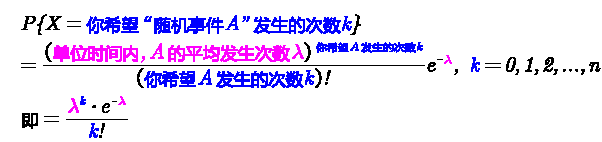
\includegraphics[width=0.8\textwidth]{/0149.pdf} \\
	上面的公式中:  \\
	- $\lambda$ : 是单位时间内, 随机事件A的\textbf{平均发生次数}. \\
	- k : 是\textbf{你希望的, 想要的} 随机事件A 发生的次数. \\
	
	
	所以, 泊松分布的``概率函数"就是: $\boxed{
		P\left(X=\text{你想要发生的次数} \right) =\frac{\text{均}^{\text{想}}\cdot e^{-\text{均}}}{\text{想!}}
	}$ \\

	记作 : $\boxed{	X \sim P(\lambda)}$	← 	即: 我们用 $Po(\lambda)$ 来表示``泊松分布". 比如, 我们将$ Y \sim Po(4)$ 读作: ``变量Y" 遵循 ``$\lambda$等于4" 的泊松分布. \\

	
	
	
	
	
	
	
	
	\begin{myEnvSample}
		``50年一遇"的大雨, 结果三年中下了两场, 这是怎么回事? \\
		其实``50年一遇"是个数学语言, 它是指: ``长期来看", 这样的大暴雨是平均50年发生一次. 注意关键词``长期". 长期是多长? 在数学中, 是指``很长很长"的时间段. \\
		所以对``长期"的理解不到位, 就是概率问题的结果``反直觉"的原因. \\
		
		平均50年发生一次, 可以是:  前4年, 每年都发生一次; 之后的196年一次都没发生. 200除以4,还是50年一次. \\
		
		所以, 我们更想知道的是: 在任何一段具体的、有限的时间内, 比如5年之内,发生1次大暴雨的概率是多少? 发生2次大暴雨的概率是多少? \\
		
		即: 当我们知道了一个随机事件A发生的概率,也知道A发生的概率符合``正态分布"之后, 那么在某一段时间或者空间间隔内,这个随机事件``发生的次数"的概率分布, 是怎样的呢? 这个问题, 就能用``泊松分布"来解决. \\
		
		泊松分布的公式是: 	$ \boxed{
		P(X=\text{你希望发生k次})=\dfrac{\lambda^k} {k!} e^{-\lambda}}$	 \\
		其中, \\
		→ \textbf{k : 为你希望``随机事件"发生的次数.} \\
		→ \textbf{$\lambda$ : 为单位时间内, 随机事件的平均发生次数.} 比如, 50年一遇的大雨 : \\
		- 如果以50年为``单位时间"的话, 发生次数就是: 1次.  ( 进一步, 我们可以算出即 : 每年发生$\frac{1} {50}$ 次).  \\
		- 如果以100年为单位的话, 发生次数就是 : 100年 ×  每年$\frac{1} {50}$次 = 2次  \\
		- 如果以5年为单位的话, 发生次数就是 :  5年 ×  每年$\frac{1} {50}$次 = 1/10次. \\ 
		
		那么套用``泊松分布公式", 来算一下, 50年中, 一次上面的大雨也不发生的概率: 即 k=0次 : \\
		
		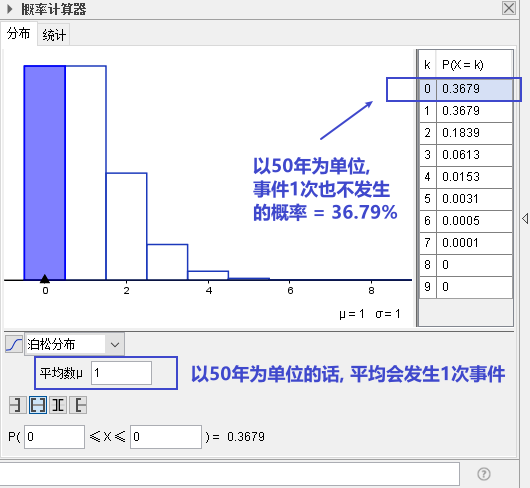
\includegraphics[width=0.75\textwidth]{/0150.png} \\
		
		再算一下 K=2, 就是接下来的``50年为单位"的话, 其中发生2次大暴雨的概率, 答案是18\%. (下图) \\
		
		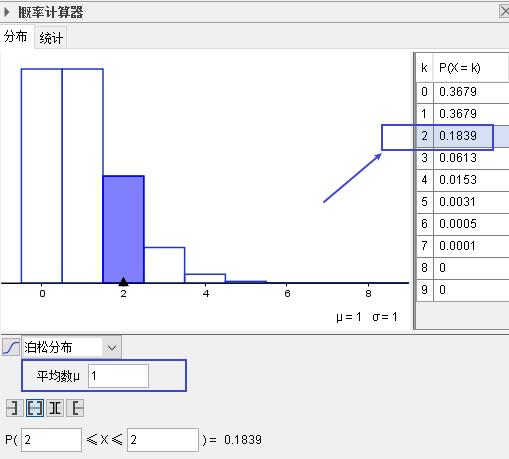
\includegraphics[width=0.75\textwidth]{/0151.png} \\	
		
		上图的右表中, 表示的就是 :  50年一遇的大雨. 你就以50年为``单位时间段" (即平均会发生一次这种大雨, 即 $\mu$ 或 $\lambda$ =1), 在这50年中, 你遇到0次, 1次, 2次, ...​ 这种大雨的真实概率, 是多少? \\
		
		50年中, 发生2次和2次以上 的概率是: 用1 减去发生0次和发生1次的概率. = 1 - (0.3679 × 2) = 26\%, 说明这并不是很小的概率事件. \\
		
		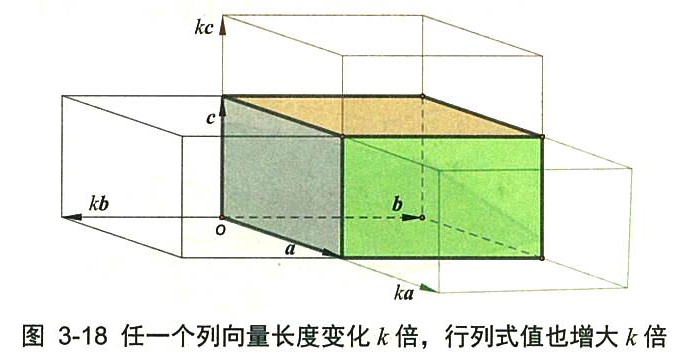
\includegraphics[width=0.75\textwidth]{/0152.png} 
	\end{myEnvSample}
	\vspace{1em} 
	
	
	
	
	\begin{myEnvSample}
		某收费站, 平均每分钟通过的车辆为3辆. 问: 1分钟内, 恰有2辆车经过的概率, 是多少? \\
		即: \\
		- 随机事件A : 收费站有车经过. \\
		- $\lambda$ (单位时间内, 随机事件平均发生的次数. 一般用 $\lambda$ 或 mean 来表示.) : 本例, 单位时间就是``每分钟", 随机事件A 发生3次. \\
		- k (你希望随机事件发生的次数. 一般用 k 或 x 来表示.) : 本例, 就是 2. (收费站有车经过, 发生2次) 
\begin{align*}  % 支持每行编号. 若不需要编号, 就用 align*环境
	&P\{X=k\}=\frac{\lambda ^k\cdot e^{-\lambda}}{k!}\\
&P\{X=\text{想\}}=\frac{\text{均}^{\text{想}}\cdot e^{-\text{均}}}{\text{想!}}=\frac{3^2e^{-3}}{2!}=0.224042
\end{align*}

	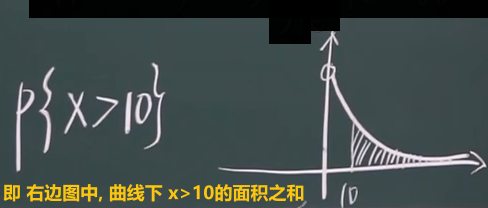
\includegraphics[width=0.5\textwidth]{/0155.png} 	
	\end{myEnvSample}
	\vspace{1em} 
	
	
	
	
	\begin{myEnvSample}
		你创建了一个关于概率的在线课程. 通常,你的学生每天问你大约4个问题, 但昨天他们问了7个. 你想知道昨天这件事, 事实上发生的可能性算多大? \\
		即 : \\
		- 随机事件A : 是学生提问. \\
		- $\lambda$ : 表示在单位时间内, 随机事件发生的平均次数. 本例就是 =4 (单位时间1天里面, 平均上, 学生提问会发生4次). \\
		- k : 你感兴趣的``随机事件发生次数". 本例就是 k=7. 
		
		即: 
		\begin{align*}  % 支持每行编号. 若不需要编号, 就用 align*环境
	&P\{X=\text{想\}}=\frac{\text{均}^{\text{想}}\cdot e^{-\text{均}}}{\text{想!}}\\
&P\{X=7\}=\frac{4^7\cdot e^{-4}}{7!}=0.0595404
		\end{align*}
	
	因此, 你收到7个问题的几率, 只有6\%. \\
	
	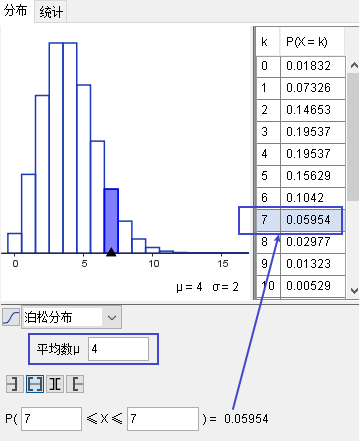
\includegraphics[width=0.55\textwidth]{/0159.png} 
	\end{myEnvSample}
	\vspace{1em} 
	
	
	
	
	
	\begin{myEnvSample}
		某航空公司, 发生事故(即随机事件A) 的平均值为: 每月 0.05次. \\
		问: \\
		→ 1年内, 发生``0事故"的概率是? \\
		随机事件, 平均每月发生0.05次, 这里的``单位时间"是以``月"为时间段的. 而问题问的是``1年内", 是以``年"为``单位时间段"的. 所以我们要统一两者的``单位时间"段. 把``月"换算成``年"来做. \\
		即: 事故的``月概率"是 0.05次, 则事故的``年概率"= 0.05 × 12 =0.6. 		
		\begin{align*}  % 支持每行编号. 若不需要编号, 就用 align*环境
	&P\{X=\text{{\color{red}想}\}}=\frac{\text{均}^{\text{{\color{red}想}}}\cdot e^{-\text{均}}}{\text{{\color{red}想}!}}\\
&P\{X=\underset{\text{随机事件在单位时间内,发生0次}}{\underbrace{{\color{red}0}}}\}=\frac{\underset{\text{事故的年概率}}{\underbrace{0.6}}^{\color{red}0}\cdot e^{-0.6}}{{\color{red}0}!}=0.548812  
		\end{align*}
	
	
		
		→ 1年内, 发生了``1次事故"的概率是? \\
		$P\{X={\color{red}1}\}=\dfrac{0.6^{\color{red}1}\cdot e^{-0.6}}{{\color{red}1}!}=0.329287$ \\
		
		
		
		→ 1年内, 发生事故 $\geq 1$次 的概率是? 
		\begin{align*}  % 支持每行编号. 若不需要编号, 就用 align*环境
	&=P\{X=2\}+P\{X=3\}+...\\
&=1-\left[ P\{X=0\}+P\{X=1\} \right]\\
& \text{把随机事件发生0次和1次的情况, 扣除掉后, 剩下的就是超过1次的所有情况了.}\\
&=1-\frac{0.6^0\cdot e^{-0.6}}{0!}-\frac{0.6^1\cdot e^{-0.6}}{1!}=0.121901
		\end{align*}
	
	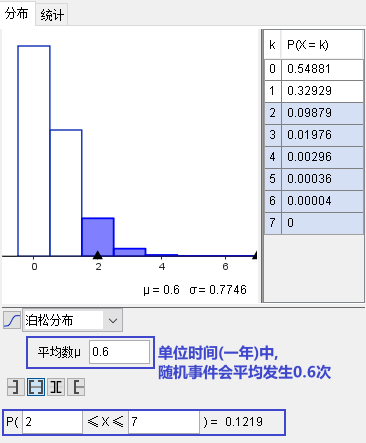
\includegraphics[width=0.55\textwidth]{/0157.png} 
	
	\end{myEnvSample}
\vspace{1em} 



\begin{myEnvSample}
	某客服工作, 每分钟收到客户来电的次数, 满足 $	X\sim P\left( \underset{\text{即}\lambda}{\underbrace{3}} \right) 	$ \\
	问: 你``每分钟收到来电不超过5次"的概率. \\
	
	即: \\
	- 随机事件A : 你收到客户来电. \\
	- $\lambda$ : 表示在单位时间(本例是1分钟)内, 随机事件发生的平均次数. 本例就是 =3. \\
	- k : 你感兴趣的``随机事件发生次数". 本例就是 $k \leq 5$.  	
	\begin{align*}  % 支持每行编号. 若不需要编号, 就用 align*环境
	&P\{X=\text{想\}}=\frac{\text{均}^{\text{想}}\cdot e^{-\text{均}}}{\text{想!}}\\
&P\{X=k\leq 5\}=\sum_{k=0}^5{\left[ P\left\{ X=k \right\} \right]}\\
&=\frac{3^0}{0!}e^{-3}+\frac{3^1}{1!}e^{-3}+...+\frac{3^5}{5!}e^{-3}=0.916
	\end{align*}
	
	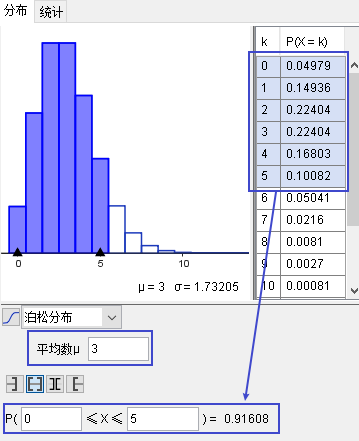
\includegraphics[width=0.55\textwidth]{/0160.png} 
	
	
\end{myEnvSample}



	
	\subsection{泊松分布的意义 ---  为我们开启了``统计推断"的大门} 
	
	连续2年下大暴雨, 这个现象是否正常? 这个问题的困难在哪儿呢? --- 数据太少. 我们没有1000年的降雨资料. 即便有,在长期、无限面前也是个渣渣, 还是太少. \\
	
	同样,物理学家要研究放射性物质的半衰期, 可绝大多数物质, 衰变期极长, 长到我们没法直接测量. 连一个完整的衰变周期都观测不到, 那怎么办呢? 用``泊松分布"解决. \\
	找一堆铋209原子,统计一下在几个确定的时间间隔中,这堆原子中有多少个发生了衰变? 只要这个数字服从``泊松分布", 反过来就证明铋209原子的衰变, 也服从``正态分布". 就可以用``正态分布"来直接计算. \\
	
	在这些问题的解决中, 统计数据, 和概率论的``概率分布 f(x)", 就被连在了一起.   \\
	而\textbf{在``泊松分布"之前, 概率和统计是两个不同的学科. ``概率"研究``未发生"的随机事件; ``统计"描述``已发生"的现实. 那会儿只有描述统计, 没有推断统计. 泊松分布开启了``推断统计"的大门, 第一次把概率和统计连接在一起.} \\
	
	
	
	
	
	\subsection{泊松分布, 其实就是``二项分布"的一种特殊情况. 当二项分布中的  n → ∞;   p→ 0 时, 我们就能用``泊松分布", 来近似该``二项分布".}
	
	当``二项分布"的n很大, 而p很小时, 我们就适合用 ``泊松分布", 来作为``二项分布"的近似.  其中λ为np. \\
	通常当$n \geq20, \ p \leq 0.05$时,就可以用``泊松公式"近似的计算. \\
	
	
	
	
	即: 当二项分布中的  n → ∞;   p→ 0 时, 我们就能用``泊松分布", 来近似该``二项分布". \\
	二项分布的``期望值", 是 $ E(X)=np=\lambda$, 所以也就是泊松分布中, $\lambda=np$. \\

	
	
	
	\begin{myEnvSample}
		某保险公司统计, 其单位时间 (1年)内, 随机事件(每位投保人发生意外死亡)的平均发生概率是 0.002. \\
		现从投保者中抽出1000人 (即 单位时间(1年)内, 这1000人里面, 会平均死亡 : 1000人 × 0.002的概率/人 = 2人 ). \\
		问: 下一年度, 会有1人死亡(而获理赔)的概率? \\
		
		这是一个二项分布 (用来描述 ``n次试验中, 事件A恰好发生k次"的概率. 即 $P\{X=k\}=C_{n}^{k}p^k(1-p)^{n-k}$). 本例中, n=1000, p=0.002. 即:\\
		$
		P\{X=\underset{\text{成功发生死亡事件\ 1人}}{\underbrace{1}}\}=C_{1000}^{1}\cdot 0.002^1\cdot (1-0.002)^{1000-1}=0.27067
		$ \\
		
		但, 由于 n很大, p很小, $np=1000×0.002=2=\lambda$, np的值适中, 我们就能用``泊松分布", 来近似``二项分布". \\
		即:
		\begin{align*}  % 支持每行编号. 若不需要编号, 就用 align*环境
			&P\{X=\text{想\}}=\frac{\text{均}^{\text{想}}\cdot e^{-\text{均}}}{\text{想!}}\\
			&P\{X=1\}=\frac{\underset{\text{均值是2人死亡}}{\underbrace{2}}^1\cdot e^{-2}}{\underset{\text{你想发生1人死亡}}{\underbrace{1}}!}=0.270671
		\end{align*}
		
		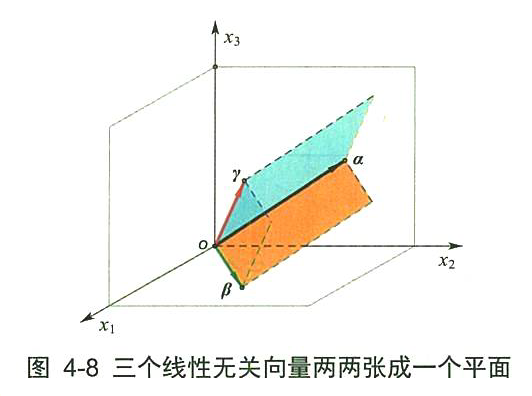
\includegraphics[width=0.55\textwidth]{/0158.png} 
	\end{myEnvSample}
	\vspace{1em} 
	
	
	
	
	\begin{myEnvSample}
		某病(非传染病), 发病率是 $\frac{1} {1000}$, 某地区有5000人, 问至少2人得病的概率? \\
		即: \\
		- 随机事件A : 有人得病. \\
		- $\lambda$ : 表示在单位空间(本例是某地区)内, 随机事件发生的平均次数. 本例就是 = 5000人 × 1/1000 = 5人. \\
		- k : 你感兴趣的``随机事件发生次数". 本例就是 ≥2人(得病).  		
		\begin{align*}  % 支持每行编号. 若不需要编号, 就用 align*环境
	&P\{X=\text{想\}}=\frac{\text{均}^{\text{想}}\cdot e^{-\text{均}}}{\text{想!}}\\
&P\{X=k\ge 2\}=1-\left[ P\left( X=0 \right) +P\left( X=1 \right) \right]\\
&=1-\frac{5^0}{0!}e^{-5}-\frac{5^1}{1!}e^{-5}=0.959572
		\end{align*}
	
	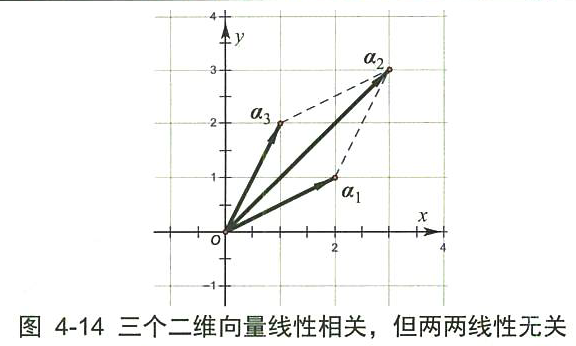
\includegraphics[width=0.6\textwidth]{/0161.png}
		
	\end{myEnvSample}
	
	
	
	
	
	
	
	\subsection{$\lambda$值越大, ``泊松分布"的曲线越对称, 越接近``正态分布"} 
	
	泊松分布所依赖的唯一参数$\lambda$, 其值越小, 分布越偏倚.  \\
	随着$\lambda$的增大, 分布越对称. \\
	当$\lambda=20$时, 接近正态分布 Normal distribution. \\
	当$\lambda \geq 50$时, 可用``正态分布"来近似处理``泊松分布"问题. \\
	
	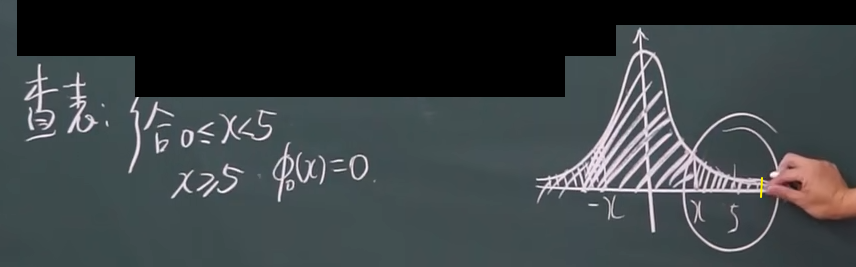
\includegraphics[width=0.6\textwidth]{/0184.png} 
	
	
	
	
	\subsection{性质 : 单位时间段越长, ``泊松分布"会向``正态分布"看齐 }
	
	随着我们把``时间单位"拉长, 我们会发现: ``泊松分布"的曲线越来越像``正态分布". \\
	
		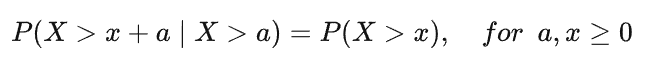
\includegraphics[width=0.6\textwidth]{/0153.png} \\	
		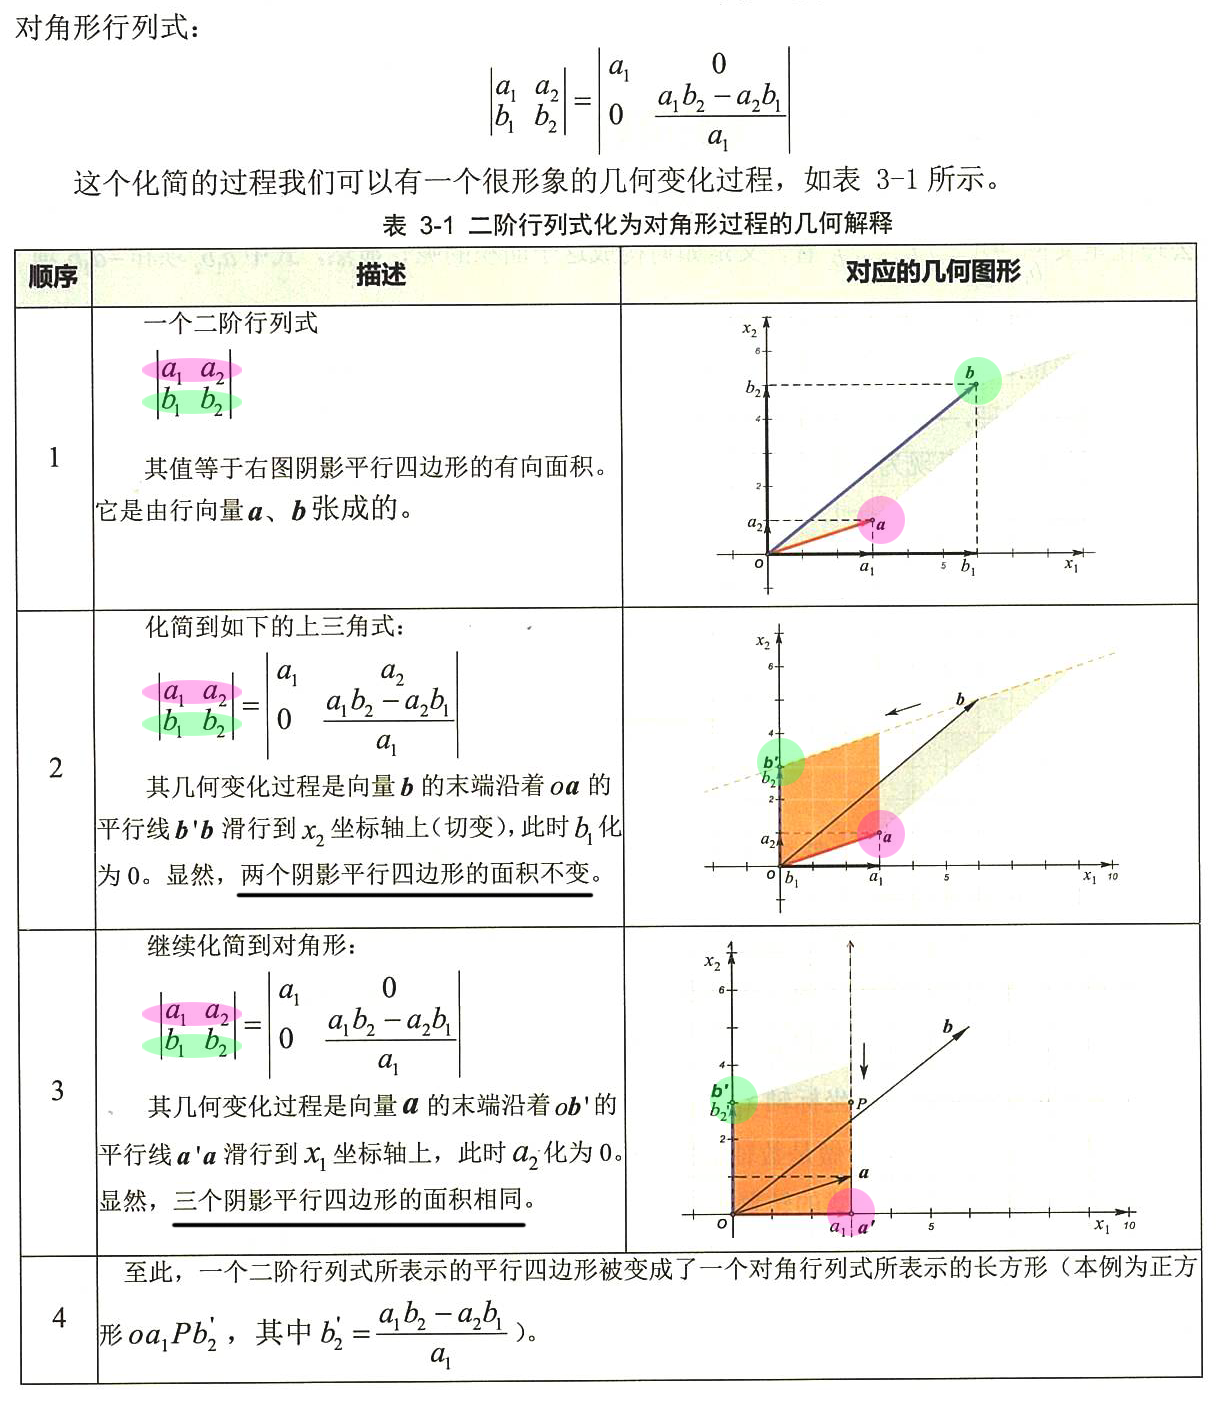
\includegraphics[width=0.6\textwidth]{/0154.png} \\	
	
	
	
	\subsection{性质 : 前后两次事件的``发生时间间隔", 无``记忆性"}
	
	泊松分布中, 事件对两次发生的时间间隔, 是无"记忆性"的. \\
	即 : 后一次事件不会记得``距离它前一次发生, 时间隔了多久". 换言之, 事件之间是相互``独立"的关系. \\
	正因此, 就一定存在一些``短间隔"和``长间隔",而很难有``一长一短、一长一短"这样有规律的出现. 否则就不叫"无记忆"了. 
	
	
	
	
	
	
\end{document}